\documentclass{beamer}
\usepackage{../../shared/styles/custom}
% =============================================================================
% ML TEACHING MATHEMATICAL NOTATION CONVENTIONS
% =============================================================================
% Based on standard ML textbooks: Murphy's "Machine Learning: A Probabilistic Perspective",
% Bishop's "Pattern Recognition and Machine Learning", and "Mathematics for Machine Learning"

% =============================================================================
% CORE NOTATION STANDARDS
% =============================================================================

% SCALARS: Regular italics (lowercase for variables, uppercase for constants)
% Examples: x, y, n, d, k, \theta, \alpha, \lambda, \sigma

% VECTORS: Bold lowercase letters
% Examples: \mathbf{x}, \mathbf{w}, \mathbf{\mu}, \mathbf{\theta}

% MATRICES: Bold uppercase letters
% Examples: \mathbf{X}, \mathbf{W}, \mathbf{\Sigma}, \mathbf{\Lambda}

% SETS: Calligraphic uppercase
% Examples: \mathcal{D}, \mathcal{X}, \mathcal{Y}

% SPACES: Blackboard bold
% Examples: \mathbb{R}, \mathbb{Z}, \mathbb{N}

% =============================================================================
% VECTOR NOTATION (bold lowercase)
% =============================================================================

\newcommand{\vx}{\mathbf{x}}        % Input vector
\newcommand{\vy}{\mathbf{y}}        % Output vector
\newcommand{\vw}{\mathbf{w}}        % Weight vector
\newcommand{\vb}{\mathbf{b}}        % Bias vector
\newcommand{\vh}{\mathbf{h}}        % Hidden vector
\newcommand{\vz}{\mathbf{z}}        % Latent vector
\newcommand{\vf}{\mathbf{f}}        % Function vector
\newcommand{\vg}{\mathbf{g}}        % Gradient vector
\newcommand{\vu}{\mathbf{u}}        % Generic vector u
\newcommand{\vv}{\mathbf{v}}        % Generic vector v
\newcommand{\vzero}{\mathbf{0}}     % Zero vector
\newcommand{\vone}{\mathbf{1}}      % Ones vector

% Greek vectors (bold)
\newcommand{\vmu}{\boldsymbol{\mu}}     % Mean vector
\newcommand{\vtheta}{\boldsymbol{\theta}} % Parameter vector
\newcommand{\vlambda}{\boldsymbol{\lambda}} % Lambda vector
\newcommand{\valpha}{\boldsymbol{\alpha}}   % Alpha vector
\newcommand{\vbeta}{\boldsymbol{\beta}}     % Beta vector
\newcommand{\vxi}{\boldsymbol{\xi}}         % Xi vector
\newcommand{\vepsilon}{\boldsymbol{\epsilon}} % Epsilon vector

% =============================================================================
% MATRIX NOTATION (bold uppercase)
% =============================================================================

\newcommand{\mX}{\mathbf{X}}        % Data matrix
\newcommand{\mY}{\mathbf{Y}}        % Target matrix
\newcommand{\mW}{\mathbf{W}}        % Weight matrix
\newcommand{\mA}{\mathbf{A}}        % Generic matrix A
\newcommand{\mB}{\mathbf{B}}        % Generic matrix B
\newcommand{\mC}{\mathbf{C}}        % Generic matrix C
\newcommand{\mH}{\mathbf{H}}        % Hidden layer matrix / Hessian
\newcommand{\mI}{\mathbf{I}}        % Identity matrix
\newcommand{\mJ}{\mathbf{J}}        % Jacobian matrix
\newcommand{\mK}{\mathbf{K}}        % Kernel matrix
\newcommand{\mL}{\mathbf{L}}        % Loss matrix / Cholesky factor
\newcommand{\mP}{\mathbf{P}}        % Projection matrix
\newcommand{\mQ}{\mathbf{Q}}        % Orthogonal matrix
\newcommand{\mR}{\mathbf{R}}        % Rotation matrix
\newcommand{\mS}{\mathbf{S}}        % Scatter matrix
\newcommand{\mU}{\mathbf{U}}        % Left singular vectors
\newcommand{\mV}{\mathbf{V}}        % Right singular vectors

% Greek matrices (bold)
\newcommand{\mSigma}{\boldsymbol{\Sigma}}   % Covariance matrix
\newcommand{\mLambda}{\boldsymbol{\Lambda}} % Diagonal eigenvalue matrix
\newcommand{\mPhi}{\boldsymbol{\Phi}}       % Feature matrix
\newcommand{\mPsi}{\boldsymbol{\Psi}}       % Basis matrix
\newcommand{\mTheta}{\boldsymbol{\Theta}}   % Parameter matrix

% =============================================================================
% SETS AND SPACES (following Bishop/Murphy conventions)
% =============================================================================

\newcommand{\cD}{\mathcal{D}}       % Dataset
\newcommand{\cH}{\mathcal{H}}       % Hypothesis space
\newcommand{\cX}{\mathcal{X}}       % Input space
\newcommand{\cY}{\mathcal{Y}}       % Output space
\newcommand{\cF}{\mathcal{F}}       % Function space
\newcommand{\cG}{\mathcal{G}}       % Gaussian process
\newcommand{\cL}{\mathcal{L}}       % Lagrangian / Loss
\newcommand{\cN}{\mathcal{N}}       % Normal distribution
\newcommand{\cU}{\mathcal{U}}       % Uniform distribution
\newcommand{\cB}{\mathcal{B}}       % Bernoulli distribution
\newcommand{\cP}{\mathcal{P}}       % Probability distribution

% Number systems
\newcommand{\Real}{\mathbb{R}}      % Real numbers
\newcommand{\Nat}{\mathbb{N}}       % Natural numbers
\newcommand{\Int}{\mathbb{Z}}       % Integers
\newcommand{\Complex}{\mathbb{C}}   % Complex numbers

% =============================================================================
% OPERATORS AND FUNCTIONS (following standard conventions)
% =============================================================================

% Prediction notation (commonly used in ML)
\newcommand{\yhat}{\hat{\vy}}        % Predicted output vector (bold)
\newcommand{\yhati}{\hat{y}_i}       % Predicted output for sample i (scalar)

% Common ML functions (with conflict resolution)
\providecommand{\sigmoid}{}
\renewcommand{\sigmoid}{\operatorname{sigmoid}}
\providecommand{\softmax}{}
\renewcommand{\softmax}{\operatorname{softmax}}
\providecommand{\ReLU}{}
\renewcommand{\ReLU}{\operatorname{ReLU}}
\providecommand{\sign}{}
\renewcommand{\sign}{\operatorname{sign}}
\DeclareMathOperator{\Gain}{Gain}    % Information gain
\DeclareMathOperator{\Entropy}{Entropy}
% KL divergence (check for conflicts)
\providecommand{\KL}{}
\renewcommand{\KL}{\operatorname{KL}}
\DeclareMathOperator{\MSE}{MSE}      % Mean squared error
\DeclareMathOperator{\MAE}{MAE}      % Mean absolute error
\DeclareMathOperator{\RMSE}{RMSE}    % Root mean squared error

% Classification metrics (upright text)
\newcommand{\TP}{\text{TP}}          % True positives
\newcommand{\TN}{\text{TN}}          % True negatives  
\newcommand{\FP}{\text{FP}}          % False positives
\newcommand{\FN}{\text{FN}}          % False negatives
\DeclareMathOperator{\Precision}{Precision}
\DeclareMathOperator{\Recall}{Recall}
\DeclareMathOperator{\Accuracy}{Accuracy}

% Transpose and inverse
\newcommand{\tp}{^\top}             % Transpose (Bishop/Murphy style)
\newcommand{\inv}{^{-1}}            % Matrix inverse
\newcommand{\pinv}{^{\dagger}}      % Pseudoinverse

% Norms (consistent with Murphy/Bishop)
\newcommand{\norm}[1]{\|#1\|}       % Generic norm
\newcommand{\normone}[1]{\|#1\|_1}  % L1 norm
\newcommand{\normtwo}[1]{\|#1\|_2}  % L2 norm
\newcommand{\norminf}[1]{\|#1\|_\infty} % L-infinity norm
\newcommand{\normF}[1]{\|#1\|_F}    % Frobenius norm

% Optimization operators (upright as in Murphy)
\providecommand{\argmin}{}
\renewcommand{\argmin}{\operatorname*{arg\,min}}
\providecommand{\argmax}{}
\renewcommand{\argmax}{\operatorname*{arg\,max}}
\DeclareMathOperator{\minimize}{minimize}
\DeclareMathOperator{\maximize}{maximize}
\DeclareMathOperator{\subjectto}{subject\,to}

% Matrix operations (upright) - use conditional definitions
\providecommand{\tr}{}
\renewcommand{\tr}{\operatorname{tr}}       % Trace
\providecommand{\det}{}
\renewcommand{\det}{\operatorname{det}}     % Determinant
\providecommand{\rank}{}
\renewcommand{\rank}{\operatorname{rank}}   % Rank
\providecommand{\span}{}
\renewcommand{\span}{\operatorname{span}}   % Span
\providecommand{\null}{}
\renewcommand{\null}{\operatorname{null}}   % Null space
\DeclareMathOperator{\range}{range} % Range/column space
\providecommand{\diag}{}
\renewcommand{\diag}{\operatorname{diag}}   % Diagonal operator
\providecommand{\vec}{}
\renewcommand{\vec}{\operatorname{vec}}     % Vectorization operator

% Probability and statistics (Murphy/Bishop style)
\newcommand{\Prob}{\mathbb{P}}      % Probability measure
\newcommand{\Exp}{\mathbb{E}}       % Expectation
\DeclareMathOperator{\Var}{Var}     % Variance
\DeclareMathOperator{\Cov}{Cov}     % Covariance
\DeclareMathOperator{\Corr}{Corr}   % Correlation
% KL divergence already defined above
\DeclareMathOperator{\MI}{I}        % Mutual information

% Activation functions (already defined above with conflict resolution)

% =============================================================================
% STANDARD PARAMETER CONVENTIONS (Murphy/Bishop style)
% =============================================================================

% Primary parameters: θ (theta) - following Murphy's convention
% Learning rates: α, η (alpha, eta)
% Regularization: λ (lambda)
% Precision: β (beta) - following Bishop
% Variance: σ² (sigma squared)
% Standard deviation: σ (sigma)
% Mean: μ (mu)

% Common scalars:
% n - number of training examples
% d - dimensionality of input
% k - number of classes/clusters
% m - number of hidden units
% T - number of time steps
% i, j - indices

% =============================================================================
% STANDARD NOTATION EXAMPLES (Murphy/Bishop style)
% =============================================================================

% Linear regression:      y = \vw\tp\vx + b
% Matrix form:            \vy = \mX\vw + b\vone
% Logistic regression:    p(y=1|\vx) = \sigmoid(\vw\tp\vx)
% Gaussian:               \vx \sim \cN(\vmu, \mSigma)
% Parameter update:       \vtheta_{t+1} = \vtheta_t - \alpha \nabla \cL(\vtheta_t)
% Likelihood:             p(\cD|\vtheta) = \prod_{i=1}^n p(y_i|\vx_i, \vtheta)
% Posterior:              p(\vtheta|\cD) \propto p(\cD|\vtheta)p(\vtheta)
% Prediction:             p(y^*|\vx^*, \cD) = \int p(y^*|\vx^*, \vtheta)p(\vtheta|\cD)d\vtheta

% =============================================================================
% COMMON MISTAKES TO AVOID
% =============================================================================

% ❌ WRONG NOTATION          →  ✅ CORRECT NOTATION (Murphy/Bishop style)

% Transpose:
% ❌ x^t, X^t              →  ✅ \vx\tp, \mX\tp
% ❌ x', X'                →  ✅ \vx\tp, \mX\tp

% Vectors vs Matrices vs Scalars:
% ❌ X (for vector)        →  ✅ \vx (bold lowercase)
% ❌ w (for weight vector) →  ✅ \vw (bold lowercase)
% ❌ x (for data matrix)   →  ✅ \mX (bold uppercase)
% ❌ \mathbf{\theta}       →  ✅ \vtheta (Greek vectors are bold)
% ❌ \mathbf{n}            →  ✅ n (scalars are not bold)

% Sets and distributions:
% ❌ R                     →  ✅ \Real (blackboard bold for number systems)
% ❌ \mathcal{R}           →  ✅ \Real (use blackboard for reals)
% ❌ Normal               →  ✅ \cN (calligraphic for distributions)

% Functions and operators:
% ❌ argmax                →  ✅ \argmax (upright operator)
% ❌ E[X]                  →  ✅ \Exp[X] (blackboard E for expectation)
% ❌ trace(A)              →  ✅ \tr(\mA) (upright operator)

% =============================================================================
% ALGORITHM NAME CONVENTIONS
% =============================================================================

% Use standard capitalizations as in textbooks:
% k-NN, SVM, PCA, GMM, EM, MAP, ML, SGD, Adam, RMSprop
% ReLU, tanh, sigmoid, softmax

\endinput

\usepackage{multicol}
%\beamerdefaultoverlayspecification{<+->}


\makeatletter
\def\magicomadjust{0em}  % a way to adjust if the spacing should be different
\newdimen\indent@amount
\def\magicom{\relax
  \ifhmode $$%
    \predisplaypenalty\@M \postdisplaypenalty\@M
    \abovedisplayskip-\baselineskip \belowdisplayskip\z@
    \abovedisplayshortskip\abovedisplayskip
    \belowdisplayshortskip\belowdisplayskip
    \global\indent@amount\predisplaysize
     $$\count@\prevgraf \advance\count@-\thr@@
         \prevgraf\count@
    \global\advance\indent@amount-2em  % correction for \predisplaysize indent
    \global\advance\indent@amount\magicomadjust  % correction for verse env, for example
    \hspace*\indent@amount
  \else\typeout{*Not in hmode*}\fi}
\makeatother




	\ifx\relax#1\relax  \item \else \item[#1] \fi
	\abovedisplayskip=0pt\abovedisplayshortskip=0pt~\vspace*{-\baselineskip}}




\title{Support Vector Machines}
\date{\today}
\author{Nipun Batra}
\institute{IIT Gandhinagar}

\begin{document}
\maketitle


{
	\setbeamercolor{background canvas}{bg=}
	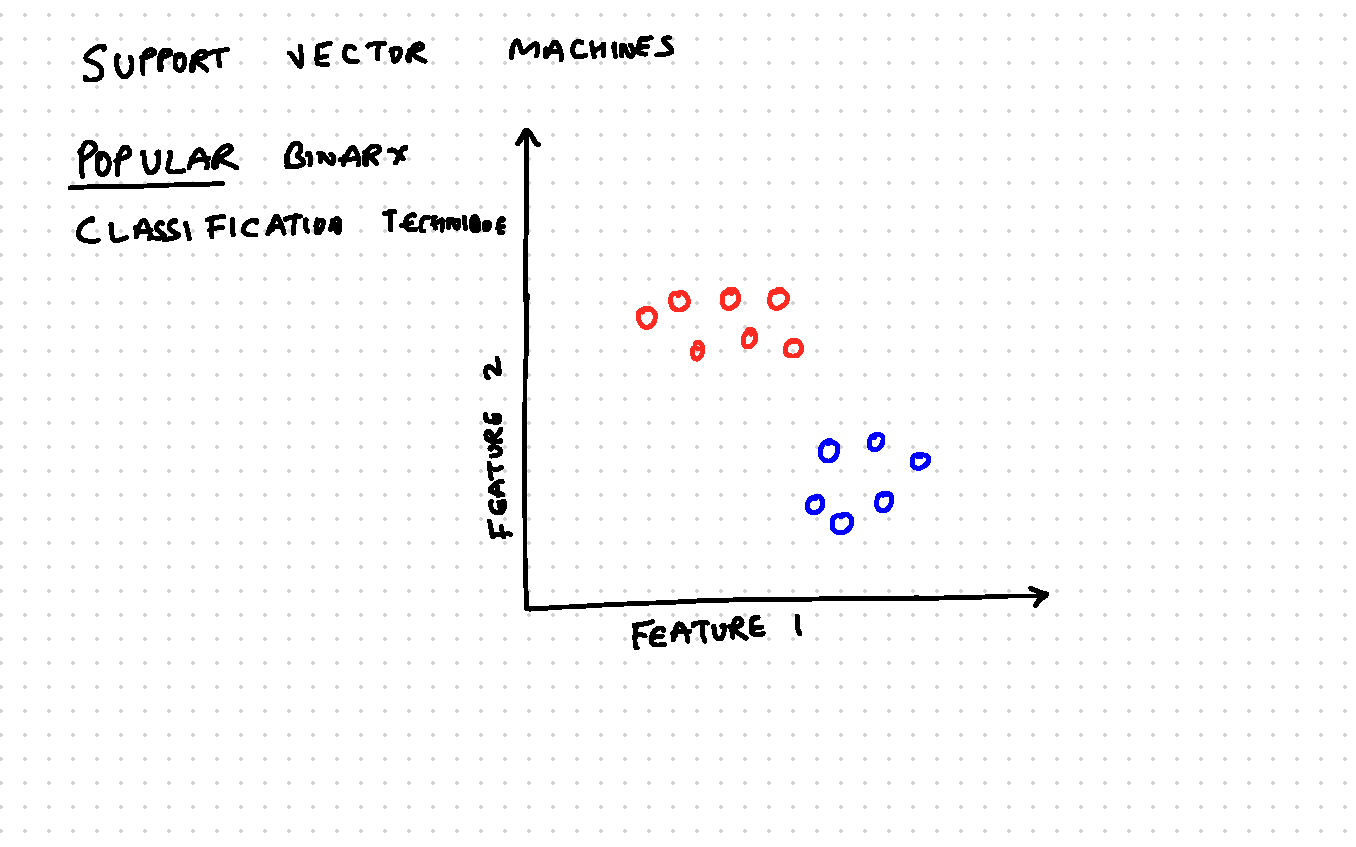
\includepdf[page=1-19]{svm/Svm-notes.pdf}
}





\begin{frame}{Distance between 2 parallel hyperplanes}
Equation of two planes is:
$$
\begin{aligned}
&\vw\cdot \vx+b_1=0\\
&\vw\cdot \vx+b_2=0
\end{aligned}
$$

\pause For a point $\vec{x_1}$ on plane 1 and $\vec{x_2}$ on plane 2, we have:
\pause $$
\begin{array}{l}
{\overrightarrow{x_{2}}=\overrightarrow{x_{1}}+t \vw} \\
{D=|t \vw|=|t|||\vw| |}
\end{array}
$$

\pause We can rewrite as follows:
\pause $$
\begin{array}{c}
{\vw \cdot \vx_{2}+b_{2}=0} \\
{\Rightarrow \vw \cdot\left(\vx_{1}+t \vw\right)+b_{2}=0}
\end{array}
$$
\pause $$
\Rightarrow \vw \cdot \vx_{1}+t\|\vw\|^{2}+b_1-b_1+b_2 = 0
\Rightarrow t = \frac{b_1 - b_2}{\|\vw\|^{2}}  \Rightarrow D = t\|\vw\| =  \frac{b_1 - b_2}{\|\vw\|}
$$
\end{frame}

{
	\setbeamercolor{background canvas}{bg=}
	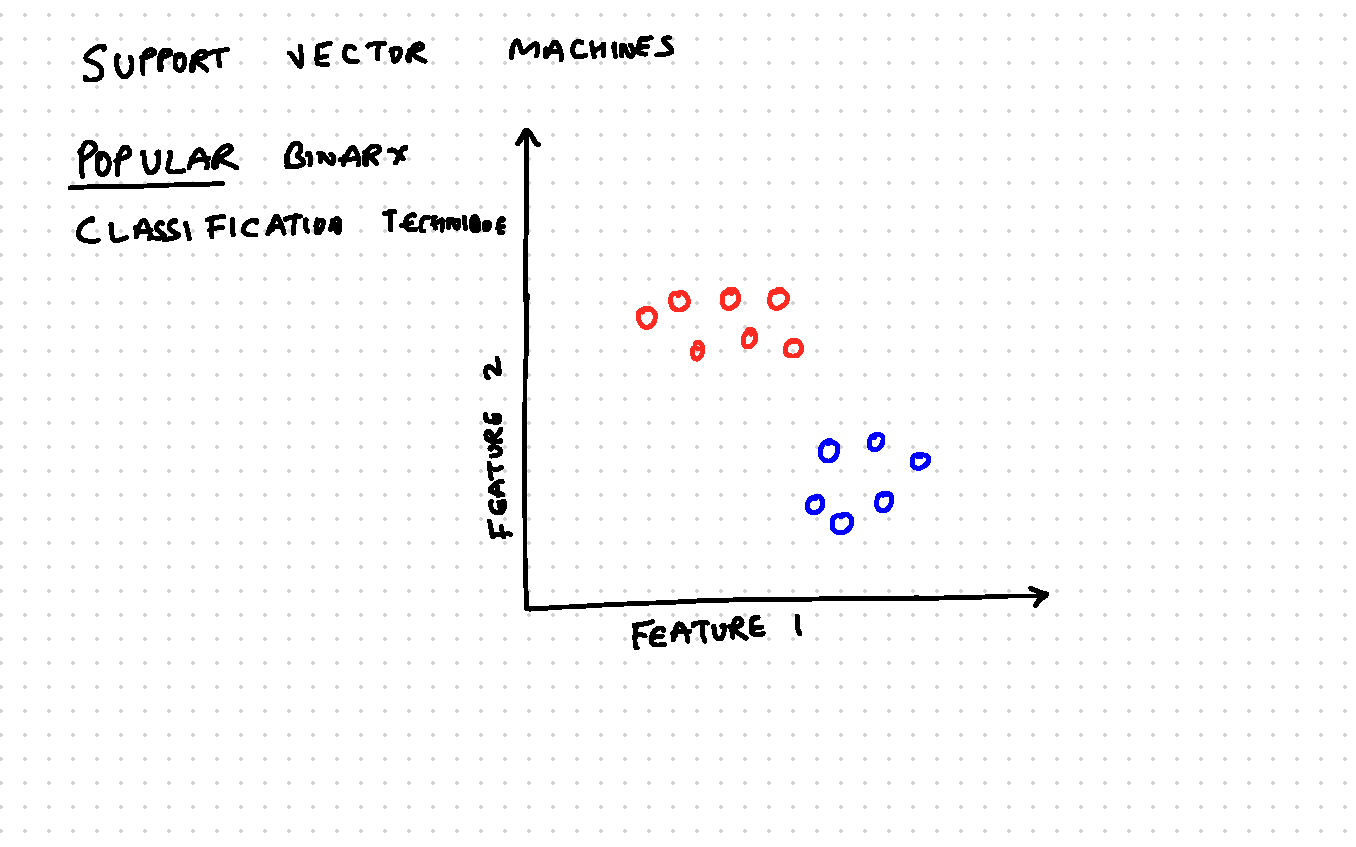
\includepdf[page=20-25]{svm/Svm-notes.pdf}
}





\begin{frame}{Primal Formulation}
	\begin{tcolorbox}{Objective}
	\begin{align*}
	\text{Minimize } & \frac{1}{2}||\vw||^{2} \\
	\text{s.t. } & y_{i}(w.x_{i} + b) \geq 1 \hspace{2mm}\forall i
	\end{align*}
\end{tcolorbox}
\pause 
Q) What is $||\vw||$?
\pause
\begin{multicols}{2}
\begin{equation*}
	 w = \begin{bmatrix}
	 w_{1} \\
     w_{2} \\
     ...  \\
     w_{n} \\
	\end{bmatrix}
\end{equation*}\break
\begin{align*}
	 ||\vw|| &= \sqrt{w^{T}w}\\
	 &= \sqrt{\begin{bmatrix}
	 w_{1}, w_{2}, ... w_{n}
	 \end{bmatrix}
	 \begin{bmatrix}
	  w_{1} \\
	  w_{2} \\
     ...  \\
     w_{n} \\
	 \end{bmatrix}}
\end{align*}

\end{multicols}

\end{frame}

{
	\setbeamercolor{background canvas}{bg=}
	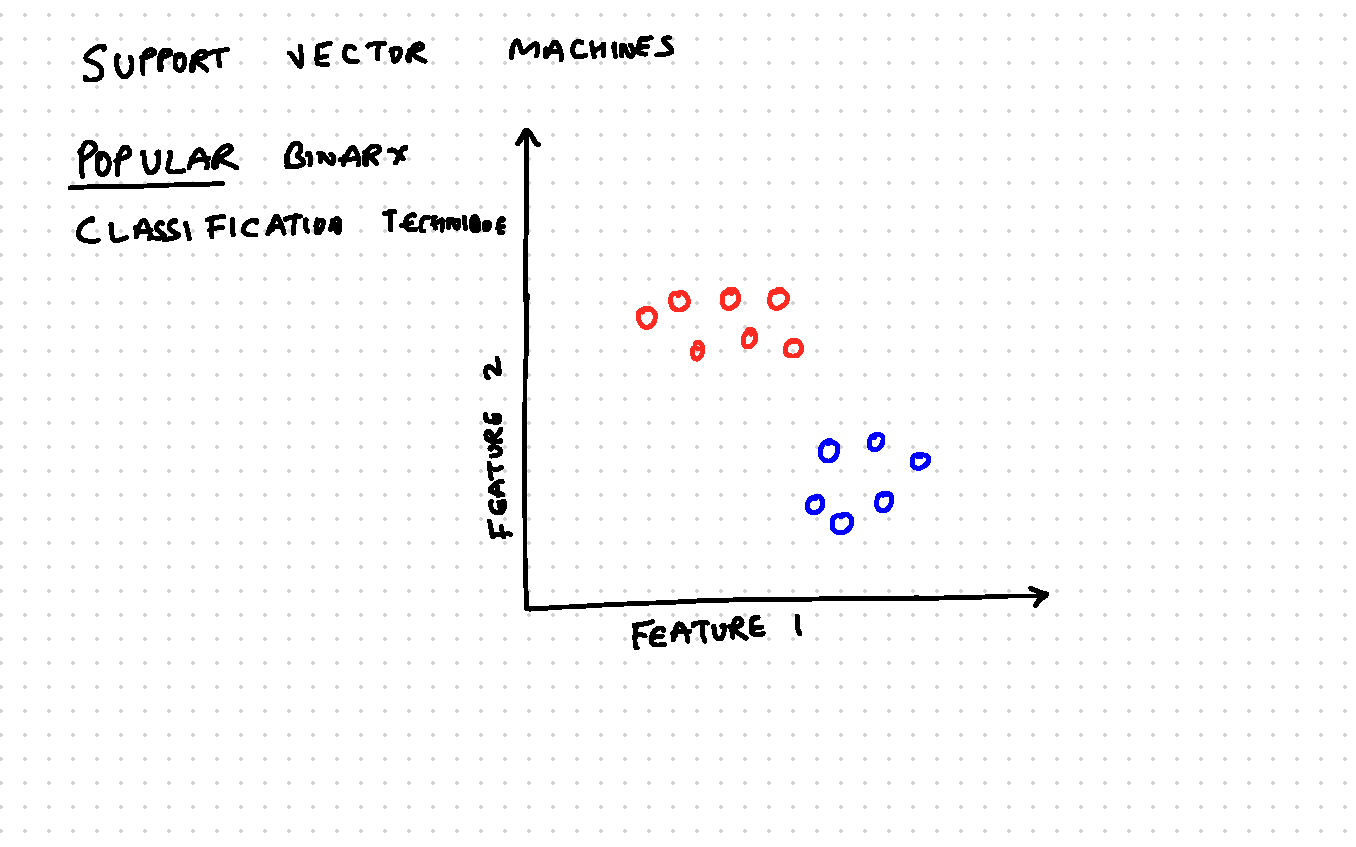
\includepdf[page=27]{svm/Svm-notes.pdf}
}



\begin{frame}{Simple Exercise}

\begin{align*}
\begin{bmatrix}
x && y \\
1 && 1\\
2 && 1\\
-1 && -1\\
-2 && -1\\
\end{bmatrix}
\end{align*}
Separating Hyperplane: $wx + b = 0$
\end{frame}

\begin{frame}{Simple Exercise}
\begin{tcolorbox}

\begin{equation*}
y_{i}(w_{i}x_{i} + b) \geq 1
\end{equation*}
\end{tcolorbox}
\begin{multicols}{2}
\begin{equation*}
\begin{bmatrix}
x_{1} && y \\
1 && 1\\
2 && 1\\
-1 && -1\\
-2 && -1\\
\end{bmatrix}
\end{equation*}\break

\begin{align*}
&\Rightarrow y_{i}(w_{i}x_{i} + b) \geq 1\\
&\Rightarrow 1(w_{1} + b) \geq 1\\
&\Rightarrow 1(2w_{1} + b)\geq 1\\
&\Rightarrow -1(-w_{1}+b) \geq 1\\
&\Rightarrow -1(-2w_{1}+b) \geq 1\\
\end{align*}


\end{multicols}
\end{frame}

{
	\setbeamercolor{background canvas}{bg=}
	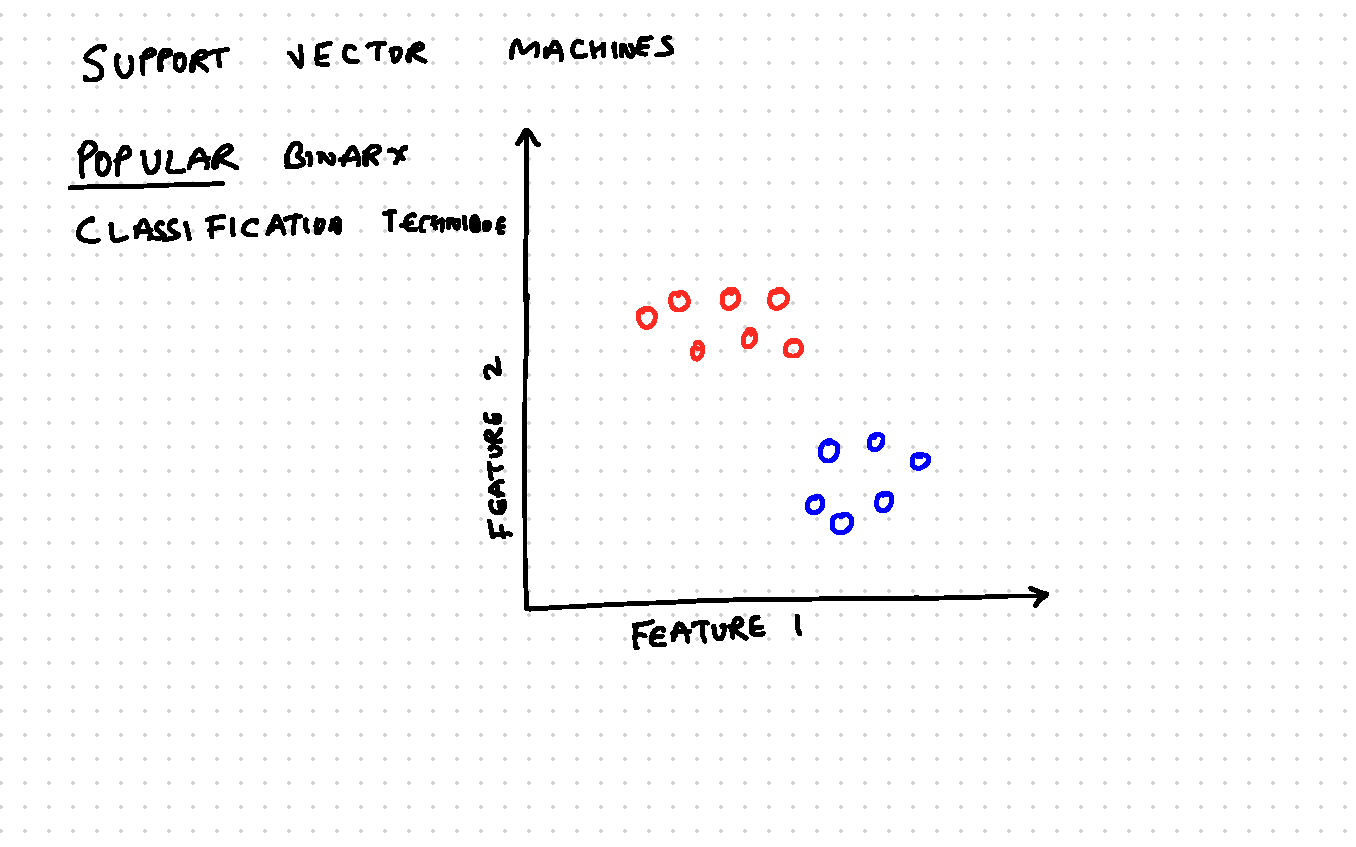
\includepdf[page=28-33]{svm/Svm-notes.pdf}
}


\begin{frame}{Simple Exercise}

\begin{align*}
w_{min} = 1, b&= 0\\
w.x + b &= 0\\
x &=0 \\
\end{align*}

\end{frame}

\begin{frame}{Simple Exercise}
Minimum values satisfying constraints  $\Rightarrow$
$w$ = 1 and $b = 0$\\
$\therefore$ Max margin classifier $ \Rightarrow x = 0$

\end{frame}

\begin{frame}{Primal Formulation is a Quadratic Program}
\begin{align*}
\text{Generally;}&\\
&\Rightarrow \text{Minimize Quadratic(x)}\\
&\Rightarrow \text{such that, Linear(x)}
\end{align*}
\begin{tcolorbox}
Question
\begin{align*}
&{x} = (x_{1}, x_{2})\\
&\text{minimize} \hspace{3mm} \frac{1}{2}||x||^{2}\\
&\colon x_{1} + x_{2} - 1 \geq 0
\end{align*}
\end{tcolorbox}
\end{frame}



{
	\setbeamercolor{background canvas}{bg=}
	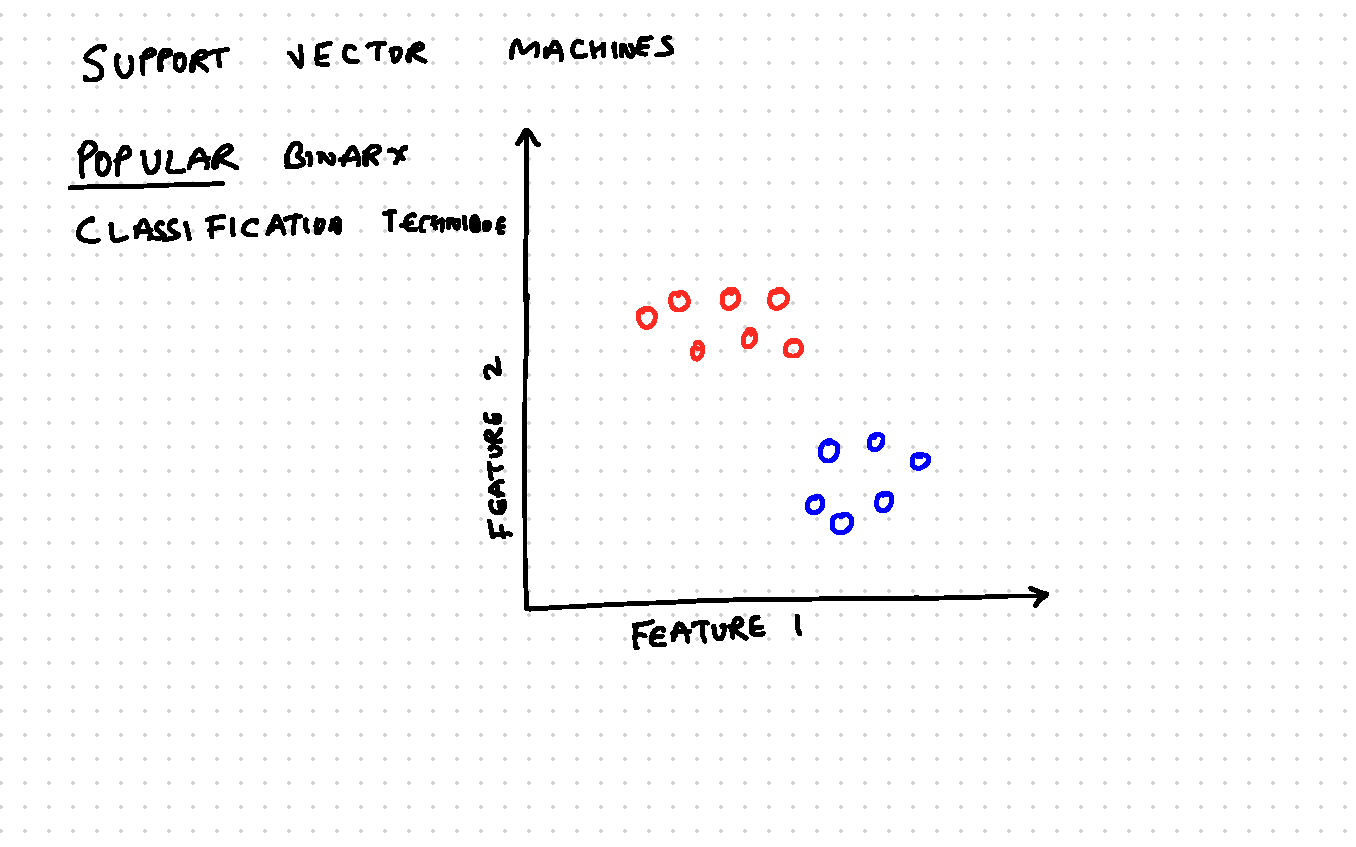
\includepdf[page=34]{svm/Svm-notes.pdf}
}



\begin{frame}{Converting to Dual Problem}
Primal $\Rightarrow$ Dual Conversion using Lagrangian multipliers\\
\begin{align*}
	\text{Minimize } & \frac{1}{2}||\bar{w}||^{2} \\
	\text{s.t. } & y_{i}(\bar{w}.x_{i} + b) \geq 1\\
	 \hspace{2mm}\forall i
	\end{align*}
\begin{align*}
&L(\bar{w},b,\alpha_{1},\alpha_{2},...\alpha_{n}) = \frac{1}{2}
\sum_{i = 1}^{d} w_{i}^{2} - \sum_{i=1}^{N} \alpha_{i}(y_{i}(\bar{w}.\bar{x_{i}} + b) - 1) \hspace{2mm} \forall \hspace{2mm}\alpha_{i} \geq 0\\
&\frac{\partial L}{\partial b} = 0 \Rightarrow \sum_{i=1}^{n}\alpha_{i}y_{i} = 0\\
\end{align*}
\end{frame}

\begin{frame}{Converting to Dual Problem}
\begin{align*}
\frac{\partial L}{\partial w} = 0 \Rightarrow & \bar{w} - \sum_{i=1}^{n}\alpha_{i}y_{i}\bar{x_{i}} = 0\\
& \bar{w} = \sum_{i=1}^{N}\alpha_{i}y_{i}\bar{x_{i}}
\end{align*}
\begin{align*}
&L(\bar{w},b,\alpha_{1},\alpha_{2},...\alpha_{n}) = \frac{1}{2}
\sum_{i = 1}^{d} w_{i}^{2} - \sum_{i=1}^{N} \alpha_{i}(y_{i}(\bar{w}.\bar{x_i} + b) -1\\
&= \frac{1}{2}||\bar{w}||^{2}-\sum_{i=1}^{N} \alpha_{i} y_{i} \vw_{.} \bar{x_{i}}-\sum_{i=1}^{N} \alpha_{i} y_{i} b+\sum_{i=1}^{N} \alpha_{i}\\
&= \sum_{=1}^{N} \alpha_{i}+\frac{\left(\sum_{i} \alpha_{i} y_{i} \bar{x}_{i}\right)\left(\sum_{j} \alpha_{j} y_{j} \bar{x}_{j}\right)}{2}-\sum_{i} \alpha_{i} y_{i}\left(\sum_{j} \alpha_{j} y_{j} \bar{x}_{j}\right) \bar{x_{i}}
\end{align*}
\end{frame}

\begin{frame}{Converting to Dual Problem}
\begin{align*}
&L(\alpha)=\sum_{i=1}^{N} \alpha_{i}-\frac{1}{2} \sum_{i=1}^{N} \sum_{j=1}^{N} \alpha_{i} \alpha_{j} y_{i} y_{j} \bar{x_{i}} \cdot \bar{x_{j}}\\
\end{align*}
\begin{tcolorbox}
\begin{align*}
&\begin{array}{ll}
{\text { Minimize }\|\bar{w}\|^{2} \Rightarrow}&{\text{Maximize } L(\alpha)} \\
{  s.t  } & {  s.t  } \\
{y_{i}\left(\bar{w}, x_{i}+b\right) \geqslant 1} & {\sum_{i=1}^{N} \alpha_{i} y_{i}=0 \hspace{2mm}\forall \hspace{2mm} \alpha_{i}  \geq 0}
\end{array}
\end{align*}
\end{tcolorbox}
\end{frame}

\begin{frame}{Question}
\textbf{Question}:\\
\vspace{2mm}
$\alpha_{i}\left(y_{i}\left(\bar{w}, \bar{x}_{i}+b\right)-1\right)=0 \quad \forall i$ as per KKT slackness\\
\vspace{2mm}
What is $\alpha_{i}$ for support vector points?\\
\vspace{4mm}
\textbf{Answer:}
For support vectors,\\
\hspace{1in}$\bar{w}.\bar{x_{i}} + b  = -1$ (+ve class)\\
\hspace{1in}$\bar{w}.\bar{x_{i}} + b  = +1$ (+ve class)\\
\vspace{2mm}
$\left.y_{i}\left(\bar{w} \cdot \bar{x}_{i}+b\right)-1\right)=0 \quad \text {for } i=\{\text{support vector points\}}$
$\therefore \alpha_{i} \text { where i } \in \text{\{support vector points\}} \neq 0$
\vspace{5mm}
$\text{For all non-support vector points }\alpha_{i} = 0$
\end{frame}

{
	\setbeamercolor{background canvas}{bg=}
	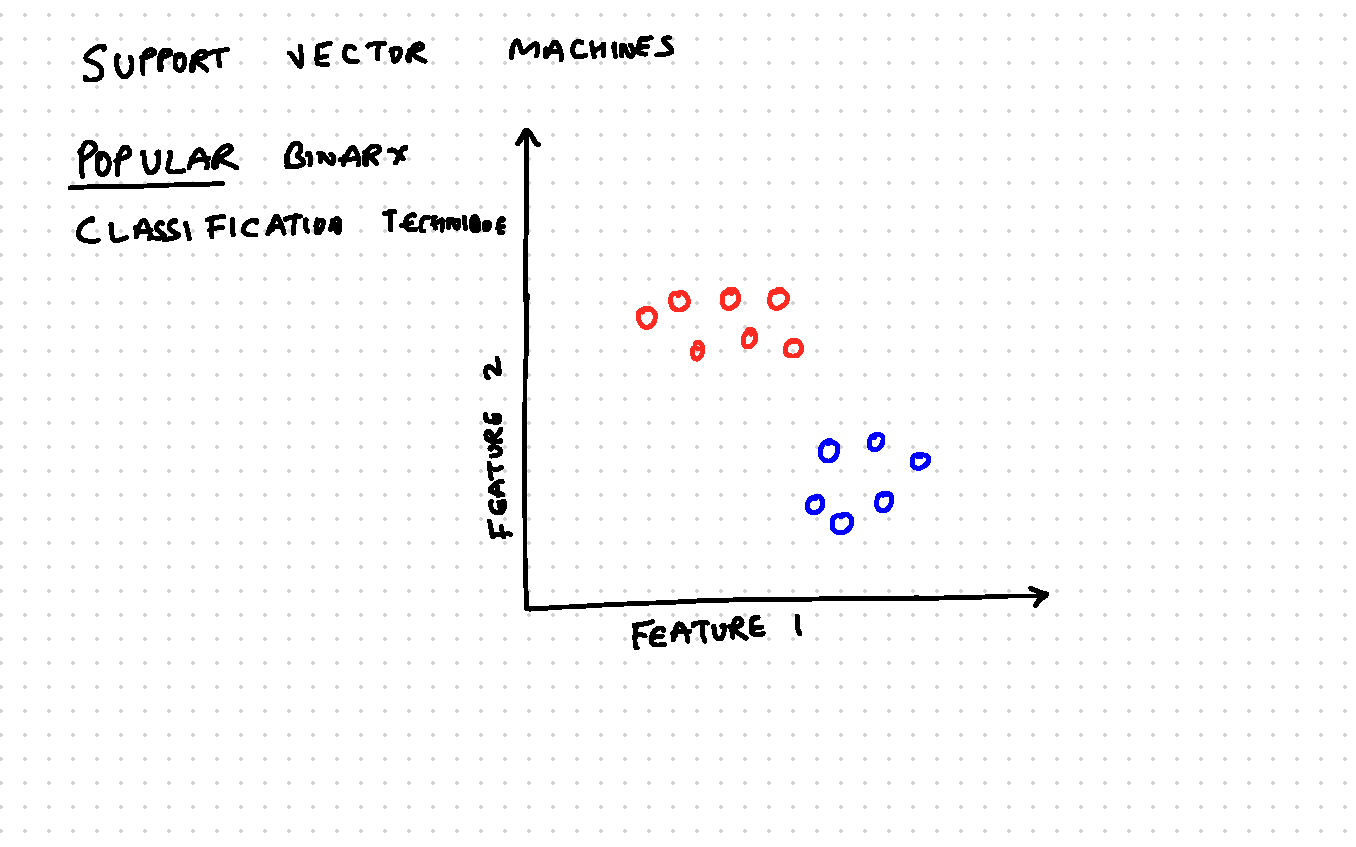
\includepdf[page=27]{svm/Svm-notes.pdf}
}


\begin{frame}{Revisiting the Simple Example}


\begin{equation*}
\begin{bmatrix}
x_{1} && y \\
1 && 1\\
2 && 1\\
-1 && -1\\
-2 && -1\\
\end{bmatrix}
\end{equation*}

\begin{align*}
L(\alpha) &= \sum_{i=1}^{4} \alpha_{i} - \frac{1}{2}\sum_{i=1}^{4}\sum_{j=1}^{4}\alpha_{i}\alpha_{j}y_{i}y_{j}\bar{x_i}\bar{x_j} \hspace{1cm}\alpha_{i} \geq 0 \\
&\sum \alpha_{i}y_{i} = 0 \hspace{1.5cm}
\alpha_{i}(y_{i}(\bar{w}.\bar{x_i} + b - 1) = 0
\end{align*}

\end{frame}

\begin{frame}{Revisiting the Simple Example}
\begin{align*}
\begin{aligned}
\left.L(\alpha_{1},\alpha_{2},\alpha_{3},\alpha_{4}\right)=& \alpha_{1}+\alpha_{2}+\alpha_{3}+\alpha_{4} \\
&-\frac{1}{2}\left\{\alpha_{1} \alpha_{1}\times(1*1) \times(1 * 1)\right.\\
&\hspace{1cm} + \\
& \alpha_{1} \alpha_{2} \times(1*1) \times(1*2) \\
&\hspace{1cm}+\\
& \alpha_{1} \alpha_{3} \times(1*-1)\times(1*1)\\
& \hspace{1cm} ... \\
& \alpha_4\alpha_4 \times(-1*-1)\times(-2*-2)
\}
\end{aligned}
\end{align*}
How to Solve? $\Rightarrow$ Use the QP Solver!!
\end{frame}

\begin{frame}{Revisiting the Simple Example}
For the trivial example, \\
We know that only x = $\pm 1$ will take part in the constraint actively. Thus, $\alpha_2, \alpha_{4} = 0$ \\
\hspace{2cm} By symmetry, $\alpha_{1} = \alpha_{3} = \alpha $\text{ (say) }\\
\hspace{2cm} \& $\sum y_i\alpha_i = 0$
\begin{align*}
\begin{aligned}
\left.L(\alpha_{1},\alpha_{2},\alpha_{3},\alpha_{4}\right)=& 2\alpha \\
&-\frac{1}{2}\left\{\alpha^{2} (1)(-1)(1)(-1) \right. \\
&\hspace{1cm} + \alpha^{2} (-1)(1)(-1)(1) \\
&\hspace{1cm} + \alpha^{2} (1)(1)(1)(1) +  \alpha^{2} (-1)(-1)(-1)(-1) \\
\}\\
\end{aligned}
\end{align*}
\hspace{2cm} $\underset{\alpha}{Maximize} \hspace{3mm} 2\alpha - \frac{1}{2}(4\alpha^{2})$
\end{frame}

\begin{frame}{Revisiting the Simple Example}
\begin{align*}
\begin{aligned}
\frac{\partial}{\partial \alpha}\left(2 \alpha- 2\alpha^{2}\right)=0 & \Rightarrow 2-4 \alpha=0 \\
\Rightarrow \hspace{2mm}& \alpha=1/2\\
\end{aligned}\\
\therefore \alpha_{1}=1/2 \hspace{2mm} \alpha_{2}=0 ; \hspace{2mm} \alpha_{3}=1/2 \hspace{2mm} \alpha_{4}=0
\\
\vw=\sum_{i=1}^{N} \alpha_{i} y_{i} \bar{x}_{i} =1/2 \times 1 \times 1+0 \times 1 \times 2 \\
+ 1/2 \times -1 \times -1 + 0\times -1 \times -2 \\
 = 1/2 + 1/2 = 1
\end{align*}
\end{frame}

\begin{frame}{Revisiting the Simple Example}
\textbf{Finding b:}\\
For the support vectors we have, \\

$y_{i}(\vw \cdot \overrightarrow{x_{i}}+b)-1=0$\\
or, $y_{i}$ $\left(\bar{w} \cdot \bar{x}_{1}+b\right)=1$\\
or, $y_{i}^{2}\left(\bar{w} \cdot \bar{x}_{i}+b\right)=y_{i}$\\
or, $\quad \bar{w}, \bar{x}_{i}+b=y_{i} \hspace{2mm}(\because y_{i}^{2} = 1)$\\
or, $b= y_i - w \cdot x_i$

In practice, $b=\frac{1}{N_{SV}} \sum_{i=1}^{N_{SV}}\left(y_{i}-\bar{w}\bar{x}_{i}\right)$

\end{frame}

\begin{frame}{Obtaining the Solution}
\begin{align*}
\begin{aligned}
b &=\frac{1}{2}\{(1-(1)(1))+(-1-(1)(-1))\\
&=\frac{1}{2}\{0+0\}=0 \\
&=0 \\
& \therefore w = 1 \hspace{2mm}\& \hspace{2mm} b = 0
\end{aligned}
\end{align*}
\end{frame}

\begin{frame}{Making Predictions}
\textbf{Making Predictions} \\
\hspace{2cm} $\hat{y}(x_i) = \operatorname{SIGN}(w \cdot x_i + b)$\\

For $x_{test} = 3$; $\hat{y}(3) = \operatorname{SIGN}(1 \times 3 + 0)$ = +ve class
\end{frame}

\begin{frame}{Making Predictions}\
\begin{align*}
\begin{array}{l}
{\text {Alternatively, }} \\
{\qquad \begin{aligned}
\hat{y}\left(x_{TEST}\right) &=\operatorname{SIGN}\left(\bar{w} \cdot \bar{x}_{TEST}+b\right) \\
&=\operatorname{SIGN} \left(\sum_{i=1}^{N_{S}} \alpha_{j} y_{j} x_{j} \cdot x_{test}+b\right)
\end{aligned}}
\end{array}
\end{align*}
\begin{align*}
\begin{aligned}
&\text{In our example,} \\
&\alpha_{1}=1/2 ; \alpha_{2}=0 ; \quad \alpha_{3}=1/2 ; \alpha_{4}=0\\
&\hat{y}(3) =\operatorname{SIGN}\left(\frac{1}{2} \times 1 \times (1 \times 3)+0+\frac{1}{2} \times (-1) \times (-1 \times 3)+0\right)\\
&=\operatorname{SIGN} \left(\frac{6}{2}\right)=\operatorname{SIGN}(3)=+1
\end{aligned}
\end{align*}

\end{frame}


\end{document}
